سیگنال پیام مجموع هفت کسینوس با فرکانس پایه‌ی $f_o = 11\ \text{kHz}$ است:
\[
x(t) = \sum_{k=1}^{7} \cos(2\pi k f_o t)
\]
پس مولفه‌های فرکانسی آن در $f_k = k f_o$ قرار دارند، یعنی:
\[
f_k \in \{11,\ 22,\ 33,\ 44,\ 55,\ 66,\ 77\}\ \text{kHz}
\]
فاصله‌ی نمونه‌برداری $T = 25\ \mu s$ است، پس فرکانس نمونه‌برداری:
\[
f_s = \frac{1}{T} = \frac{1}{25\times 10^{-6}} = 40\ \text{kHz}
\]

نمونه‌برداری توسط قطار ضربه، طیف را تکرار می‌کند؛ تبدیل فوریه‌ی سیگنال نمونه‌برداری‌شده برابر است با:
\[
X_s(f) = \frac{1}{T}\sum_{n=-\infty}^{\infty} X\big(f - n f_s\big)
\]
بنابراین هر مولفه‌ی $f_k$ به‌همراه همه‌ی نسخه‌های جابه‌جاشده‌ی $f_k \pm n f_s$ ظاهر می‌شود. مولفه‌ای که در باند پایه ($|f| \leq f_s/2 = 20\ \text{kHz}$) دیده می‌شود، فرکانس آلیاس‌شده است:
\[
f_k^{\text{alias}} = \big|\,f_k - n\,f_s\,\big|_{\min}
\qquad (\text{نزدیک‌ترین مضرب } f_s = 40\ \text{kHz})
\]

سپس خروجی از فیلتر پایین‌گذر ایده‌آل با پهنای باند $16\ \text{kHz}$ عبور می‌کند؛ پس تنها مولفه‌هایی با $f_k^{\text{alias}} < 16\ \text{kHz}$ باقی می‌مانند. جدول زیر فرکانس آلیاس و سرنوشت هر مولفه را نشان می‌دهد:
\begin{center}
\begin{LTR}
\begin{tabular}{|c|c|c|c|}
\hline
$k$ & $f_k$ (kHz) & $f_k^{\text{alias}}$ (kHz) & فیلتر $16\,$kHz \\
\hline
$1$ & $11$ & $|11-0|=11$  & عبور \\
$2$ & $22$ & $|22-40|=18$ & حذف \\
$3$ & $33$ & $|33-40|=7$  & عبور \\
$4$ & $44$ & $|44-40|=4$  & عبور \\
$5$ & $55$ & $|55-40|=15$ & عبور \\
$6$ & $66$ & $|66-80|=14$ & عبور \\
$7$ & $77$ & $|77-80|=3$  & عبور \\
\hline
\end{tabular}
\end{LTR}
\end{center}

تنها مولفه‌ی $k=2$ (با آلیاس $18\ \text{kHz} > 16\ \text{kHz}$) توسط فیلتر حذف می‌شود و بقیه باقی می‌مانند. بنابراین خروجی فیلتر مجموع شش کسینوس با فرکانس‌های زیر است (با فرض بهره‌ی فیلتر بازسازی $T$ که دامنه‌ها را حفظ می‌کند):
\[
y(t) = \cos(2\pi\!\cdot\!3t) + \cos(2\pi\!\cdot\!4t) + \cos(2\pi\!\cdot\!7t)
     + \cos(2\pi\!\cdot\!11t) + \cos(2\pi\!\cdot\!14t) + \cos(2\pi\!\cdot\!15t)
\]

تبدیل فوریه‌ی خروجی، مجموعه‌ای از ضربه‌ها در فرکانس‌های باقی‌مانده است؛ هر کسینوس با دامنه‌ی $1$ به دو ضربه با ارتفاع $\tfrac{1}{2}$ تبدیل می‌شود:
\[
Y(f) = \frac{1}{2}\!\!\sum_{f_i \in \{3,4,7,11,14,15\}}\!\!\big[\delta(f - f_i) + \delta(f + f_i)\big]
\qquad (\text{kHz})
\]
یعنی ۱۲ ضربه با ارتفاع $\tfrac{1}{2}$ در $f = \pm 3,\ \pm 4,\ \pm 7,\ \pm 11,\ \pm 14,\ \pm 15\ \text{kHz}$ و هیچ مولفه‌ای در $\pm 18\ \text{kHz}$ وجود ندارد. نمودار این طیف در شکل زیر رسم شده است:

\begin{center}
\IfFileExists{figs/1.png}
  {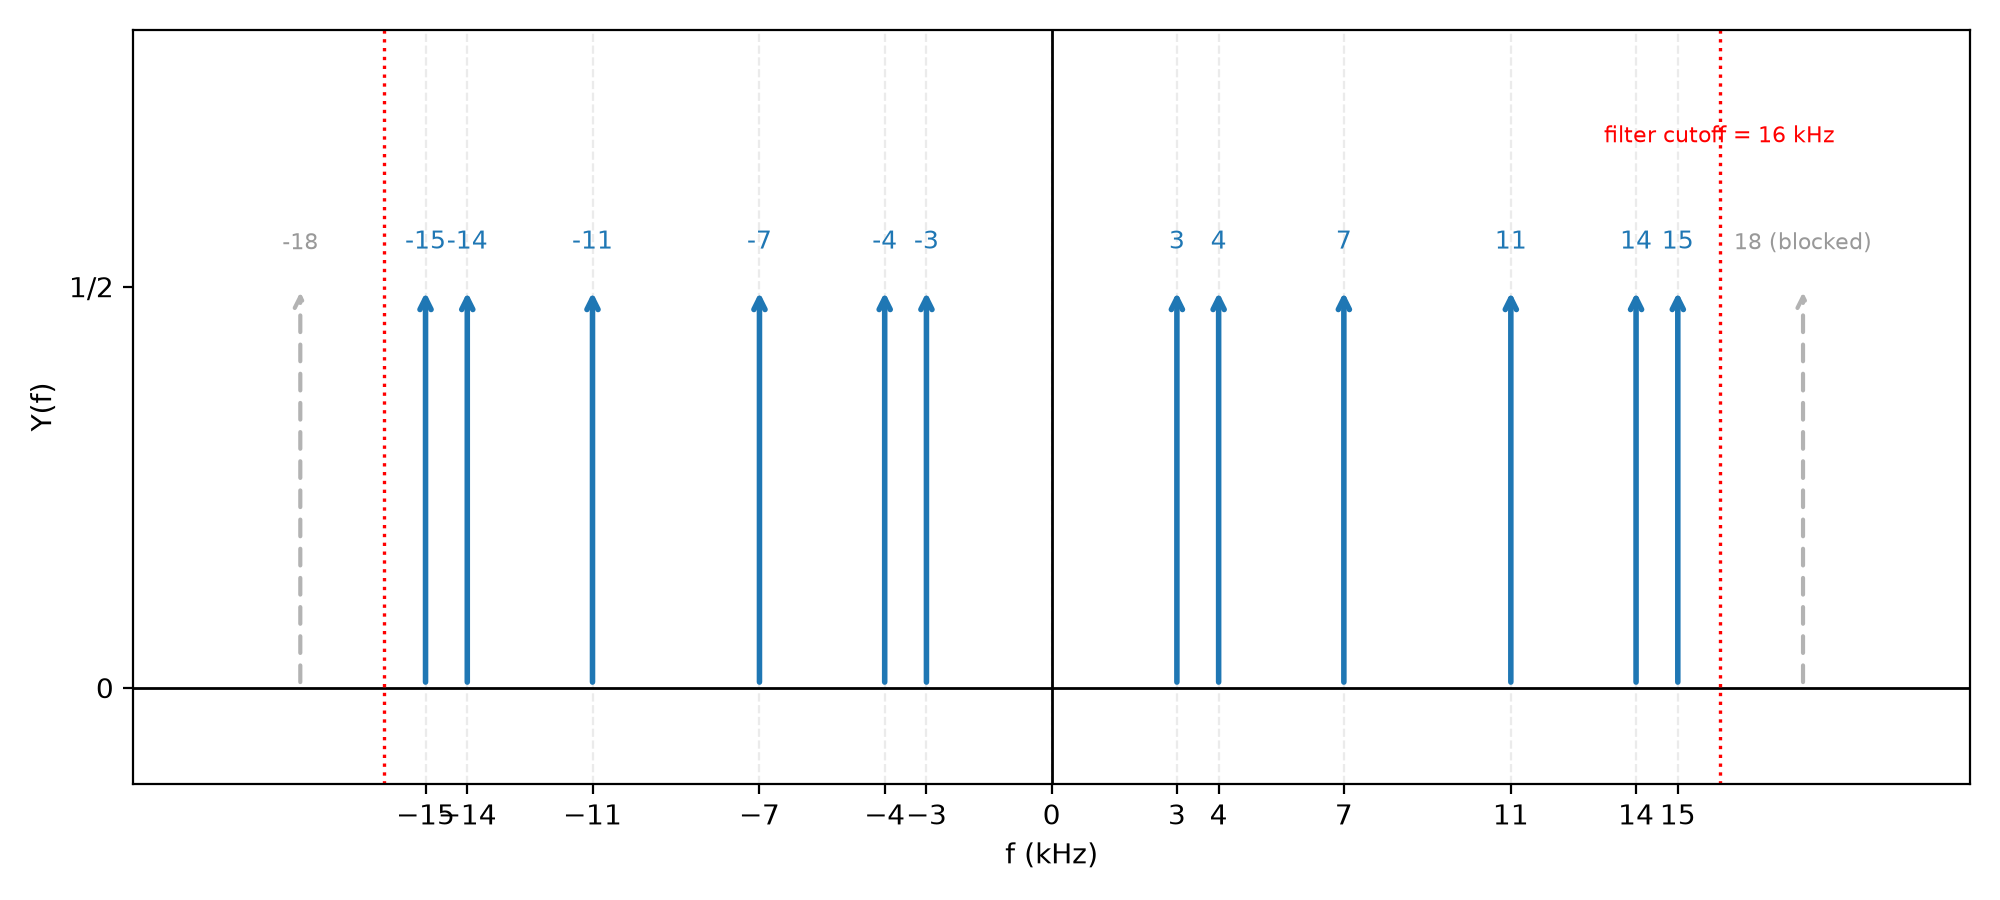
\includegraphics[width=1\textwidth]{figs/1.png}}
  {\fbox{\parbox{0.8\textwidth}{\centering \vspace{2em} «جای نمودار طیف خروجی $Y(f)$ — تصویر در \lr{figs/1.png} قرار گیرد» \vspace{2em}}}}
\end{center}
